\section*{Question 1 --- Inverted pendulum}
\answer{(a) State-space model}
With $x=[\theta,\dot\theta]^\mathsf{T}$, input $u$ and output $y=\theta$,
\begin{equation}
 \dot x_1=x_2,\qquad
 \dot x_2=19.62\sin x_1-x_2+20\cos x_1\,u,\qquad y=x_1.
\end{equation}
The Simulink plant uses two Integrators and the gravity, friction and input terms above. Initial state: $x(0)=[0.1,0]^\mathsf{T}$ (rad, rad/s).

\answer{(b) Input-output linearization and validity}
Differentiating $y$ twice exposes $u$:
\begin{equation}
 \ddot y=19.62\sin\theta-\dot\theta+20\cos\theta\,u.
 \qquad
 \boxed{u=\frac{0.05v-0.981\sin\theta+0.05\dot\theta}{\cos\theta}.}
\end{equation}
Then $\ddot y=v$. The new states remain $z_1=\theta$, $z_2=\dot\theta$, with $\dot z_1=z_2$, $\dot z_2=v$. Relative degree equals the state dimension; there are no internal dynamics. The law requires $\cos\theta\ne0$; around upright its connected domain is $|\theta|<\pi/2$. Required input can grow near the boundary.

\answer{(c) Linear regulation: approximately 1 s settling}
Choose $v=-k_p\theta-k_d\dot\theta$. Matching a repeated pole at $-6$ gives
\begin{equation}
 s^2+k_ds+k_p=(s+6)^2,
 \qquad \boxed{k_p=36,\quad k_d=12.}
\end{equation}
The exact response is $\theta(t)=0.1(1+6t)e^{-6t}$. Thus $(1+6T_s)e^{-6T_s}=0.02$ gives $T_s=0.9723$ s, with no overshoot.

\answer{(d) Closed-loop simulation}
\begin{center}
$\boxed{\text{Linear state feedback}}\xrightarrow{v}
\boxed{\text{Nonlinear cancellation}}\xrightarrow{u}
\boxed{\text{Pendulum}}$\\[2pt]
\small Measured $\theta,\dot\theta$ feed both controllers.
\end{center}
The simple model is \texttt{part1\_pendulum\_regulation.slx}. Run for 2 s using \texttt{ode45}, maximum step 0.005 s, relative/absolute tolerances $10^{-8}/10^{-10}$. The Angle, Rate, Acceleration and Input scopes observe the loop.
\begin{center}
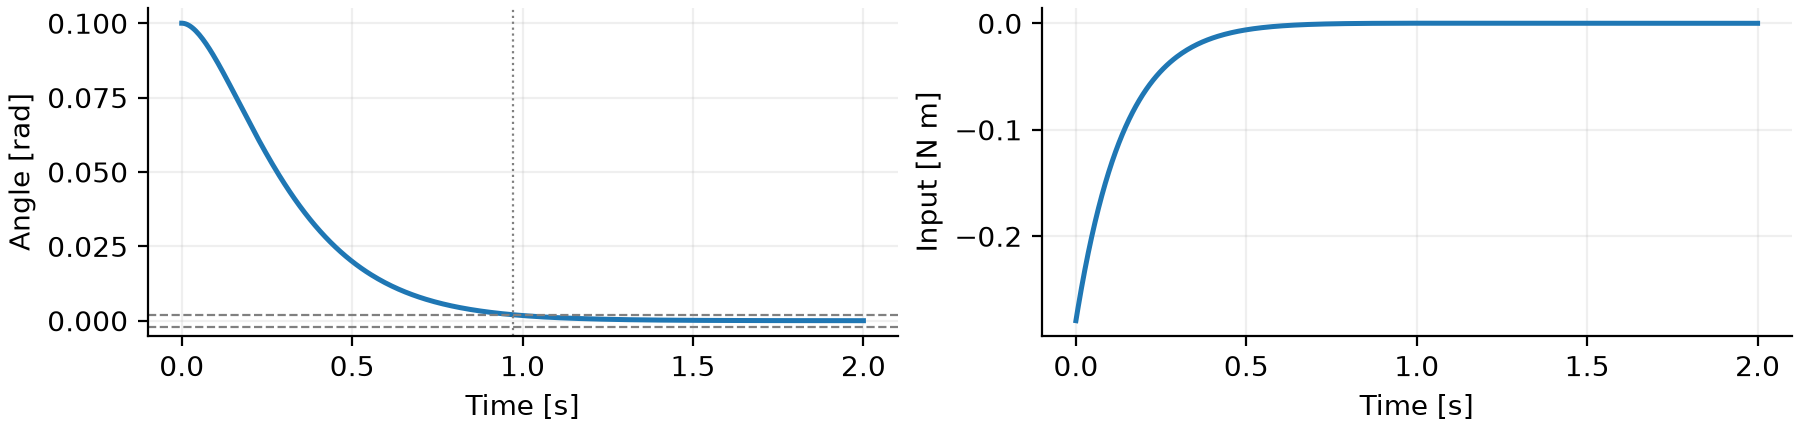
\includegraphics[width=\linewidth]{report_pendulum_response.png}
\reportcaption{Logged simulation signals; the dashed band is $\pm0.002$ rad. The schematic above is explanatory, not a UI screenshot.}
\end{center}
The sampled 2\% settling time is \textbf{0.9762 s}, satisfying the approximate 1 s requirement. Peak $|u|=0.2793$ N\,m. Seven validation cases passed; the largest angle discrepancy from the analytical response was $1.37\times10^{-11}$ rad. These results assume exact cancellation and unconstrained input; no hardware test is claimed.
